\chapter{Linux Commands \\
\small{\textit{-- Charles, Justin, Benedict, Jacky}}
\index{Linux Commands} 
\index{Chapter!Linux Commands}
\label{Chapter::Linux Commands}}

\section{Part A: Navigation \& File Ops}
\begin{itemize}
    \item 1: 
        \begin{lstlisting}[language=Python]
(base) jackylei@Jackys-MacBook-Pro lx-test % pwd
/Users/jackylei/lx-test
        \end{lstlisting}
    \item 2: 
        \begin{lstlisting}[language=Python]
(base) jackylei@Jackys-MacBook-Pro lx-test % ls -a -lh
total 136
drwxr-xr-x@ 12 jackylei  staff   384B Sep 15 16:56 .
drwxr-x---+ 58 jackylei  staff   1.8K Sep 13 22:14 ..
-rw-r--r--@  1 jackylei  staff   6.0K Sep 15 16:53 .DS_Store
drwxr-xr-x@  3 jackylei  staff    96B Sep 15 16:52 archive
-rw-r--r--@  1 jackylei  staff    48K Sep 13 22:14 blob.bin
lrwxr-xr-x@  1 jackylei  staff    13B Sep 13 22:14 link-to-file1 -> src/file1.txt
-rw-r--r--@  1 jackylei  staff     0B Sep 15 16:56 notes.md
-rw-r--r--@  1 jackylei  staff    56B Sep 15 16:56 people.csv
drwxr-xr-x@  5 jackylei  staff   160B Sep 13 22:14 src
-rw-r--r--@  1 jackylei  staff    56B Sep 13 22:14 sys.log
drwxr-xr-x@  3 jackylei  staff    96B Sep 15 16:04 tmp
-rw-r--r--@  1 jackylei  staff    28B Sep 13 22:14 words.txt
        \end{lstlisting}
    \item 3: 
        \begin{lstlisting}[language=Python]
(base) jackylei@Jackys-MacBook-Pro lx-test % [ -d tmp ] && cp -v src/file1.txt tmp
src/file1.txt -> tmp/file1.txt
        \end{lstlisting}
    \item 4: 
        \begin{lstlisting}[language=Python]
(base) jackylei@Jackys-MacBook-Pro lx-test % mv -v old.txt archive/
old.txt -> archive/old.txt
        \end{lstlisting}
    \item 5: 
        \begin{lstlisting}[language=Python]
(base) jackylei@Jackys-MacBook-Pro lx-test % touch notes.md
        \end{lstlisting}
    \item 6:     
        \begin{lstlisting}[language=Python]
(base) jackylei@Jackys-MacBook-Pro lx-test % du -h src
        \end{lstlisting}
\end{itemize}

\section{Part B: Viewing \& Searching}
\begin{itemize}
    \item 7: 
        \begin{lstlisting}[language=Python]
(base) jackylei@Jackys-MacBook-Pro lx-test % cat -n sys.log
     1	INFO boot ok
     2	WARN disk low
     3	ERROR fan fail
     4	INFO shutdown
        \end{lstlisting}
    \item 8:
        \begin{lstlisting}[language=Python]
(base) jackylei@Jackys-MacBook-Pro lx-test % cat sys.log | grep "ERROR"
ERROR fan fail
        \end{lstlisting}
    \item 9:
        \begin{lstlisting}[language=Python]
(base) jackylei@Jackys-MacBook-Pro lx-test % grep -o -i '[[:alnum:]]\+' words.txt | sort -u | wc -l
       4
        \end{lstlisting}
    \item 10:
        \begin{lstlisting}[language=Python]
(base) jackylei@Jackys-MacBook-Pro lx-test % cat words.txt | grep -i "g"
Gamma
gamma
        \end{lstlisting}
    \item 11:
        \begin{lstlisting}[language=Python]
(base) jackylei@Jackys-MacBook-Pro lx-test % head -2 people.csv
id,name,dept
1,Ada,EE
        \end{lstlisting}
    \item 12:
        \begin{lstlisting}[language=Python]
(base) jackylei@Jackys-MacBook-Pro lx-test % tail -3 sys.log
WARN disk low
ERROR fan fail
INFO shutdown
        \end{lstlisting}
\end{itemize}

\section{Part C: Text Processing}
\begin{itemize}
    \item 13: 
        \begin{lstlisting}[language=Bash]
awk -F ',' 'NR > 1 {print $2}' people.csv
        \end{lstlisting}

        \begin{figure}[H]
            \centering
            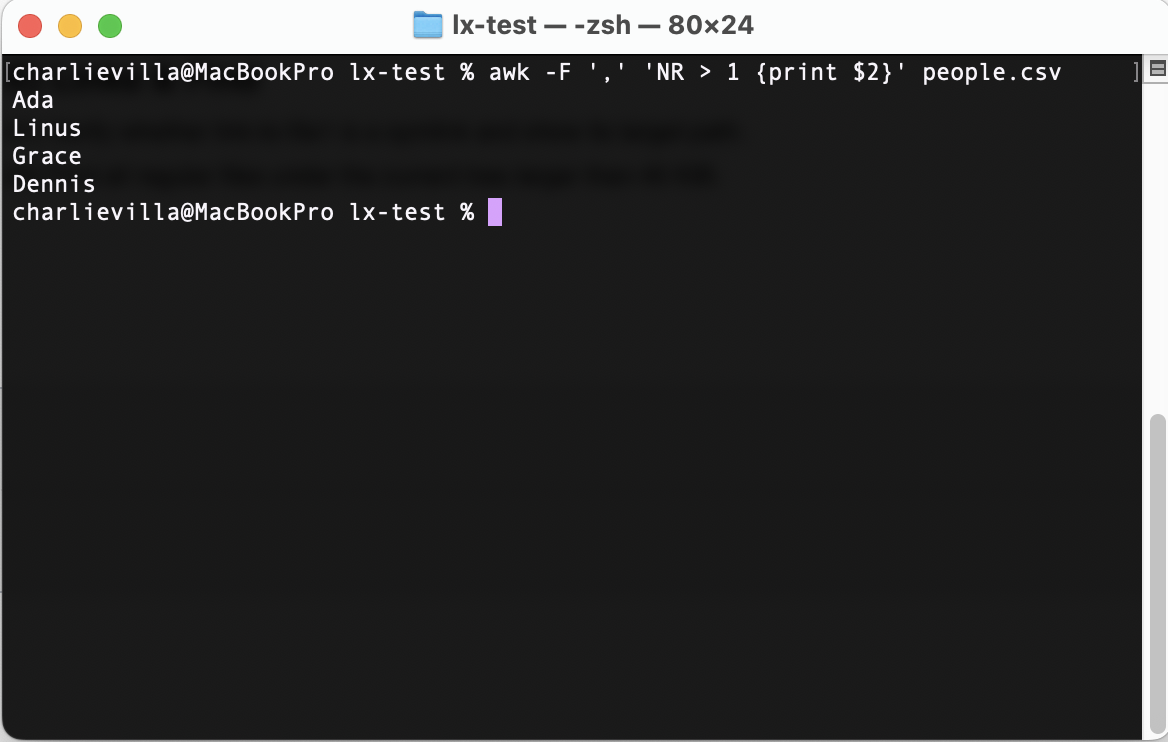
\includegraphics[width=15cm, height=10cm]{png/LinuxProblemSetPicsPNG/part_c_13.png}
            \caption{Part C \#13 Terminal Output}
            \label{fig:part C 13}
        \end{figure}
    \item 14: 
        \begin{lstlisting}[language=Bash]
sort -f -u words.txt
        \end{lstlisting}

        \begin{figure}[H]
            \centering
            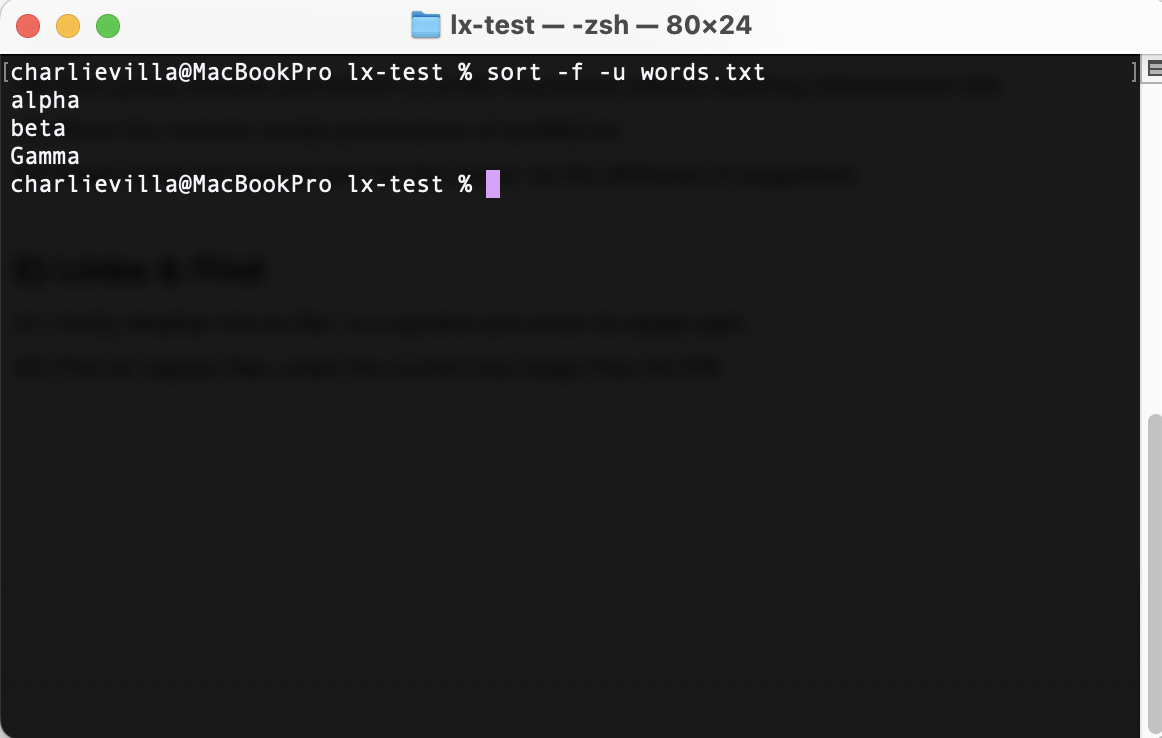
\includegraphics[width=15cm, height=10cm]{png/LinuxProblemSetPicsPNG/part_c_14.png}
            \caption{Part C \#14 Terminal Output}
            \label{fig:part C 14}
        \end{figure}
    \item 15: 
    \begin{lstlisting}[language=Bash]
find src/ -type f -exec sed -i.bak 's/three/3/g' {} +
    \end{lstlisting}

    No terminal output for question 15
    \item 16: 
        \begin{lstlisting}[language=Bash]
wc src/*.txt
        \end{lstlisting}

        \begin{figure}[H]
            \centering
            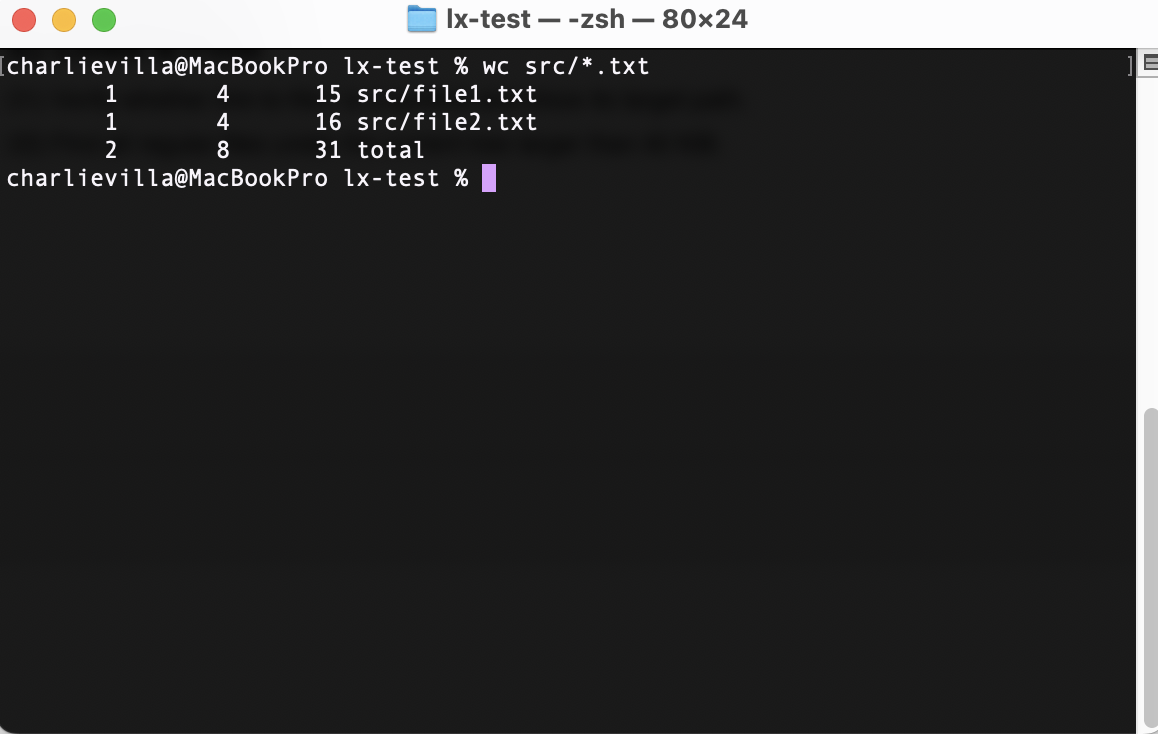
\includegraphics[width=15cm, height=10cm]{png/LinuxProblemSetPicsPNG/part_c_16.png}
            \caption{Part C \#16 Terminal Output}
            \label{fig:partC 16}
        \end{figure}
\end{itemize}

\section{Part D: Permissions \& Ownership}
\begin{itemize}
    \item 17: 
        \begin{lstlisting}[language=Bash]
chmod 700 tmp/
        \end{lstlisting}

        No terminal output for question 17
    \item 18: 
        \begin{lstlisting}[language=Bash]
chmod -R g+x src/lib
        \end{lstlisting}

        No terminal output for question 18
    \item 19: 
    \begin{lstlisting}[language=Bash]
stat -f %p src/file2.txt
    \end{lstlisting}

    \begin{figure}[H]
        \centering
        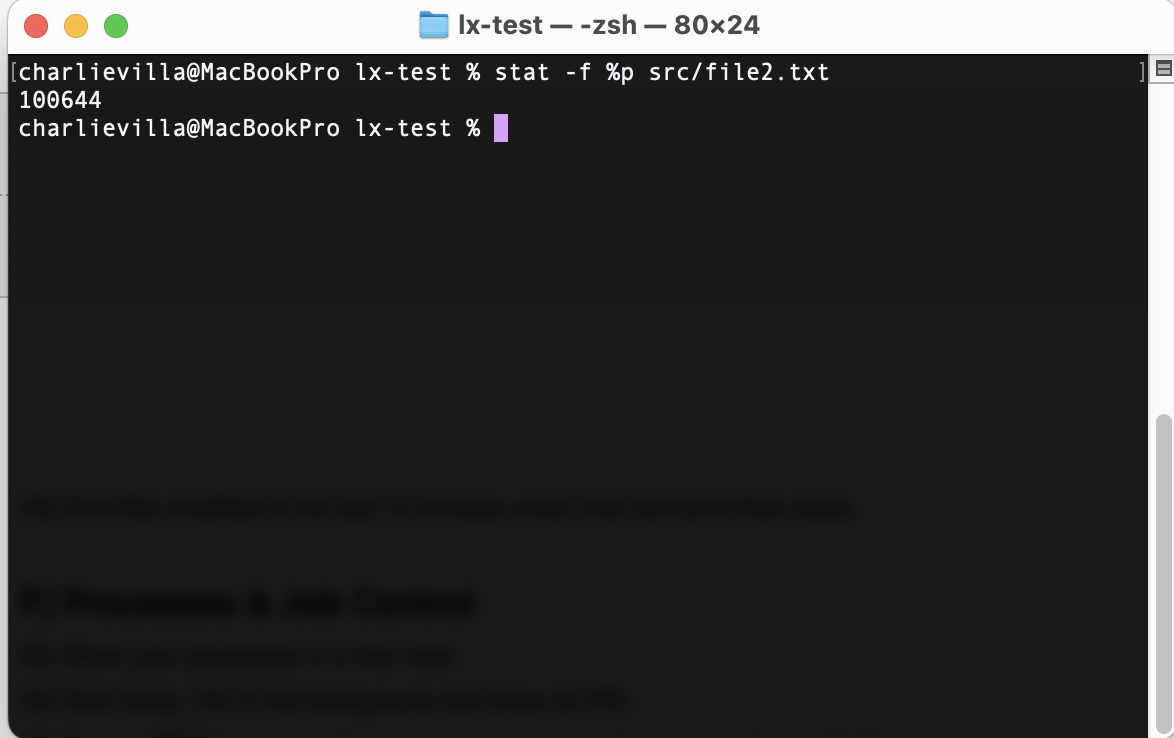
\includegraphics[width=15cm, height=10cm]{png/LinuxProblemSetPicsPNG/part_d_19.png}
        \caption{Part C \#19 Terminal Output}
        \label{fig:partC 19}
    \end{figure}
    \item 20: 
    \begin{lstlisting}[language=Bash]
touch notes.md
chflags uappnd notes.md
    \end{lstlisting}

    No terminal output for question 20
\end{itemize}

\section{Part E: Links \& Find}
\begin{itemize}
    \item 21: 
    \begin{lstlisting}[language=Bash]
ls -l link-to-file1
    \end{lstlisting}

    \begin{figure}[H]
        \centering
        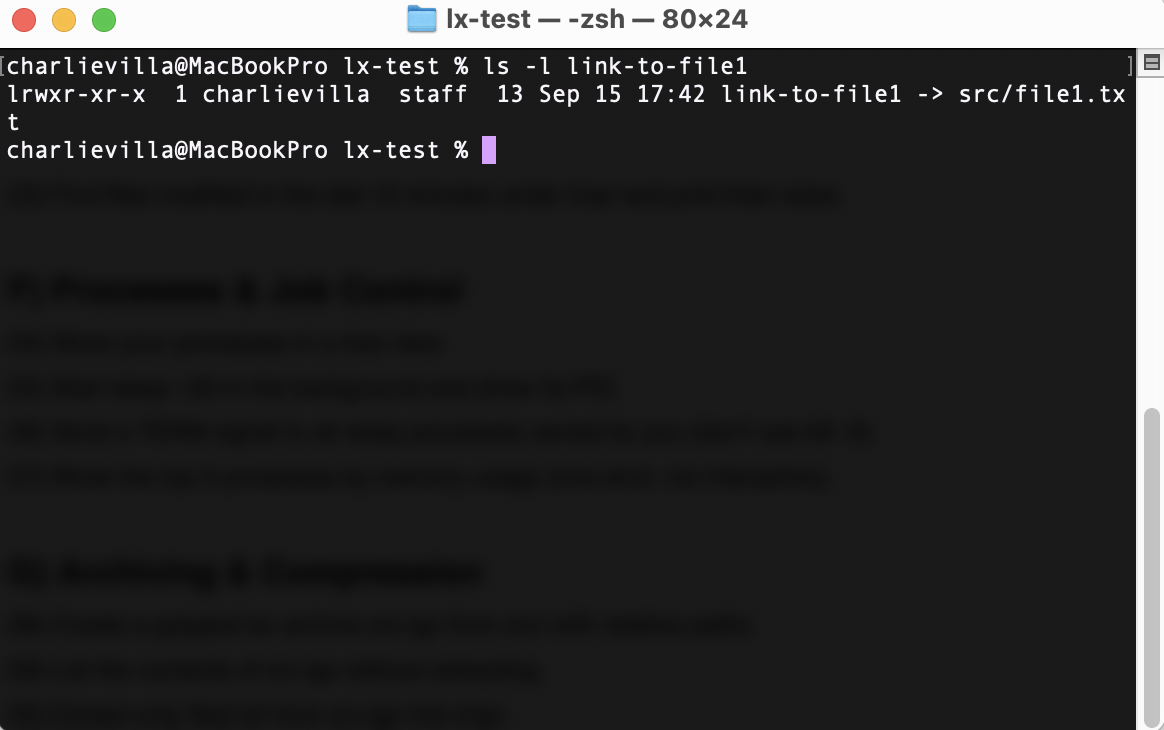
\includegraphics[width=12cm, height=7cm]{png/LinuxProblemSetPicsPNG/part_e_21.png}
        \caption{Part C \#21 Terminal Output}
        \label{fig:partC 21}
    \end{figure}    
    \item 22: 
    \begin{lstlisting}[language=Bash]
find . -type f -size +40k
    \end{lstlisting}

    \begin{figure}[H]
        \centering
        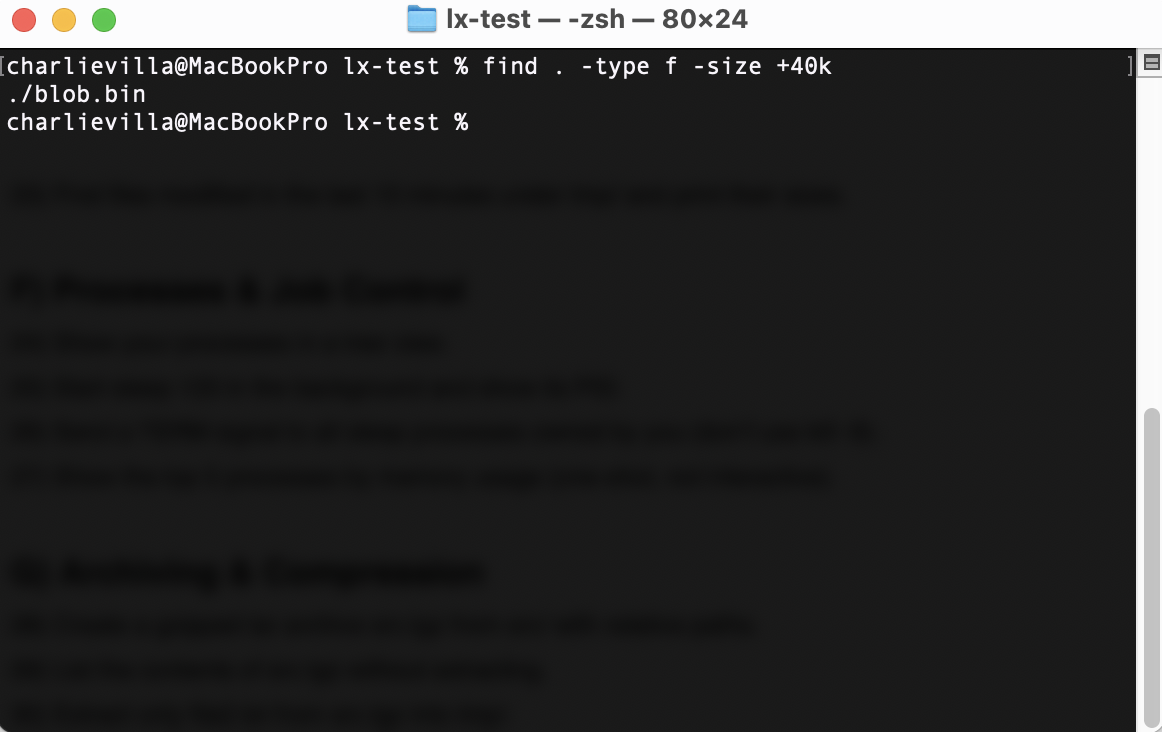
\includegraphics[width=12cm, height=7cm]{png/LinuxProblemSetPicsPNG/part_e_22.png}
        \caption{Part C \#22 Terminal Output}
        \label{fig:partC 22}
    \end{figure}  
    \item 23: 
    \begin{lstlisting}[language=Bash]
touch tmp/some-new-file.txt
find tmp/ -type f -mmin -10 -exec stat -f "%z %N" {} +
    \end{lstlisting}

    Created a new file with "touch" because the tmp/ directory was empty before it.

    \begin{figure}[H]
        \centering
        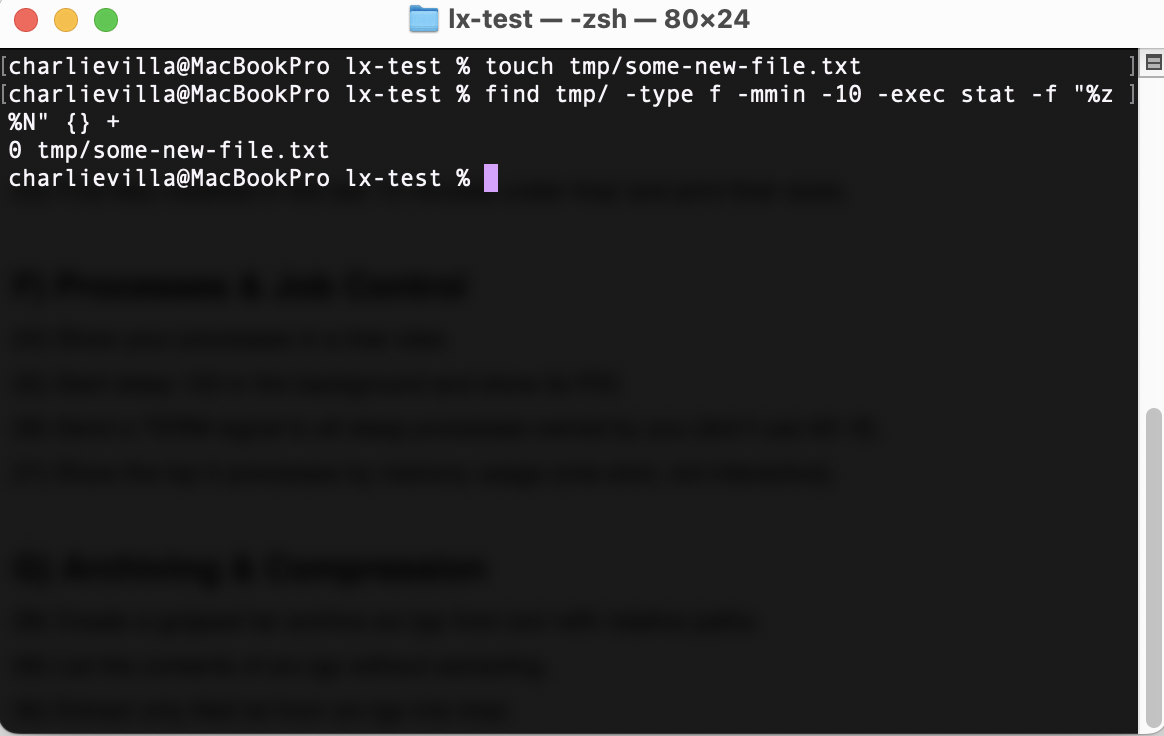
\includegraphics[width=12cm, height=7cm]{png/LinuxProblemSetPicsPNG/part_e_23.png}
        \caption{Part C \#23 Terminal Output}
        \label{fig:partC 23}
    \end{figure}  
\end{itemize}

\section{Part F: Processes \& Job Control}
\begin{itemize}
    \item 24: Tree View:
    \begin{figure}[H]
        \centering
        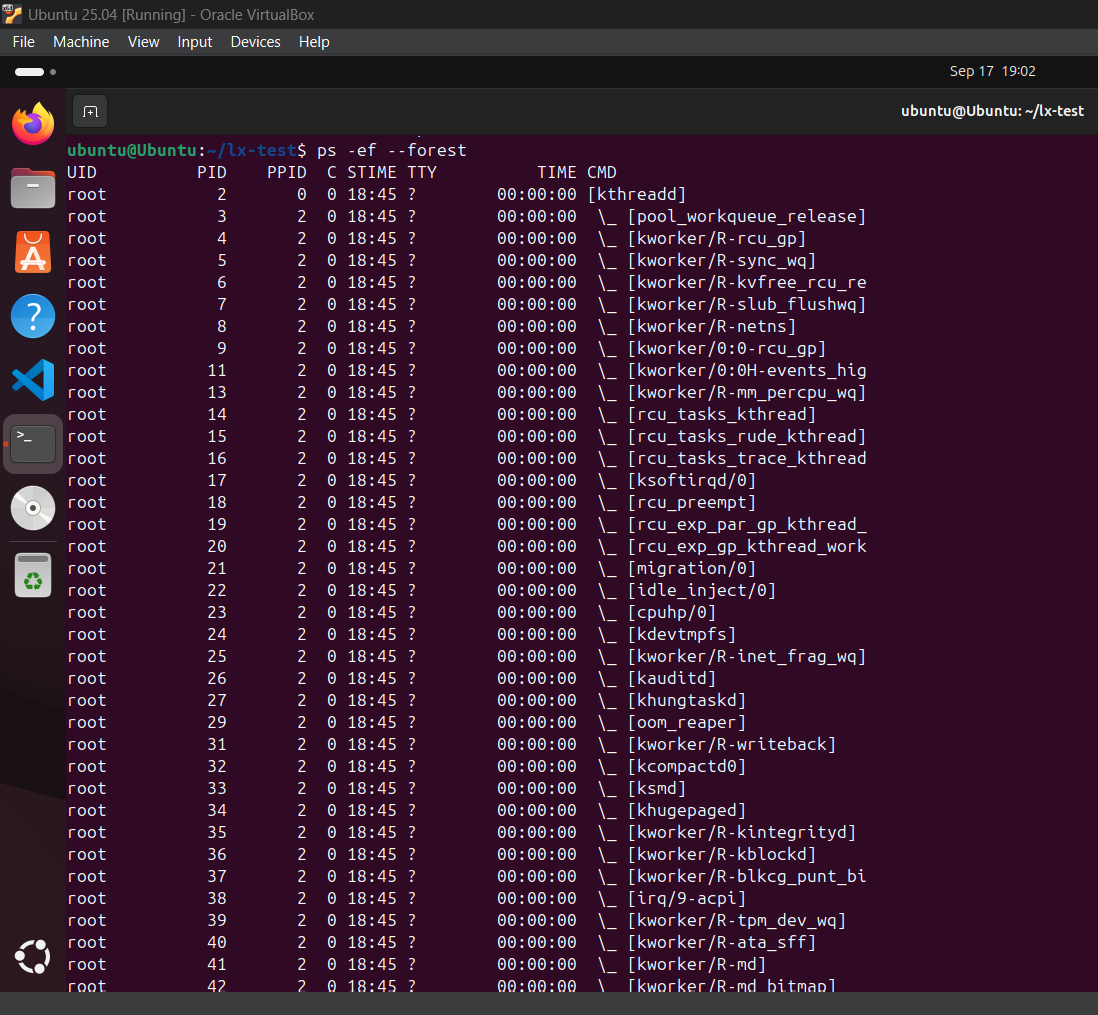
\includegraphics[width=15cm, height=10cm]{png/LinuxProblemSetPicsPNG/TreeView1.png}
        \caption{Part F \#24 Tree View 1}
        \label{fig:partF 24 Tree 1}
    \end{figure}
    \begin{figure}[H]
        \centering
        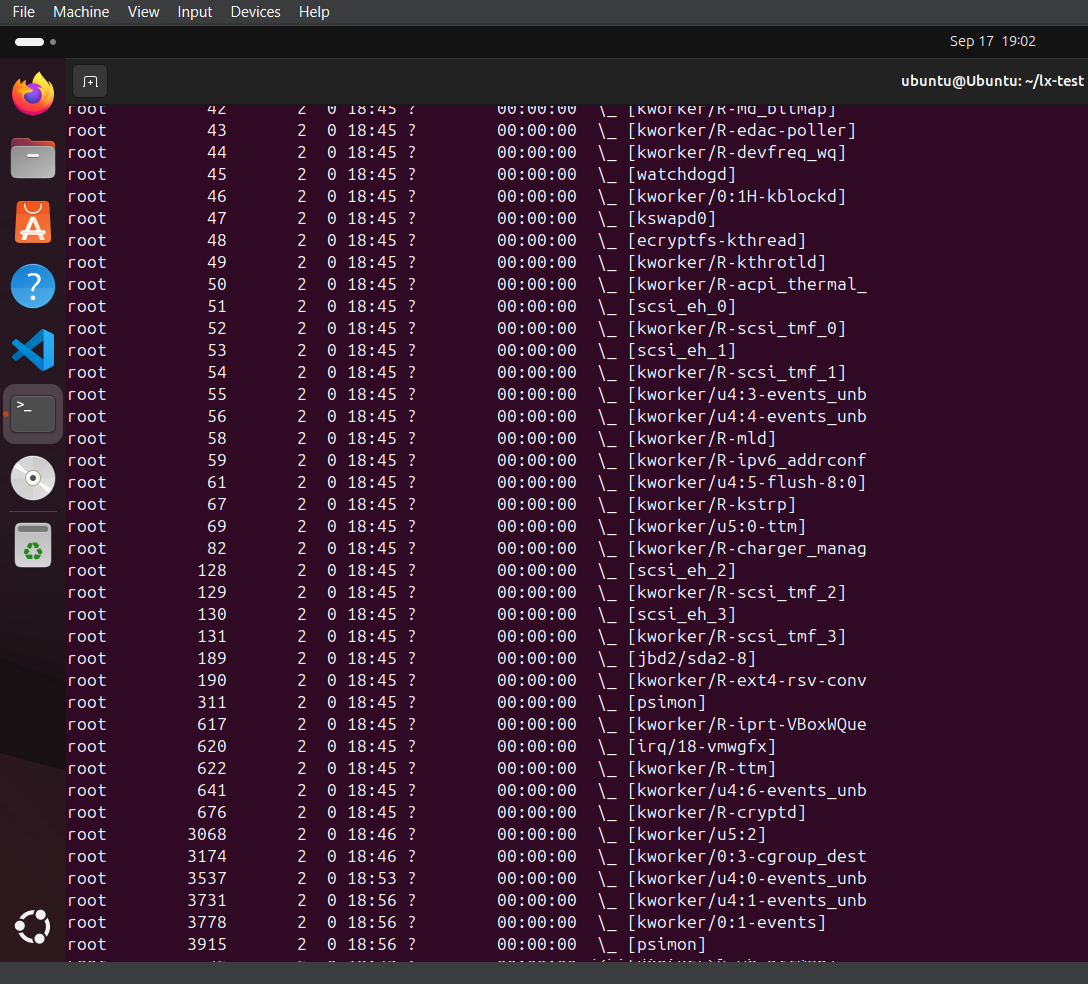
\includegraphics[width=15cm, height=10cm]{png/LinuxProblemSetPicsPNG/TreeView2.png}
        \caption{Part F \#24 Tree View 2}
        \label{fig:partF 24 Tree 2}
    \end{figure}
    \begin{figure}[H]
        \centering
        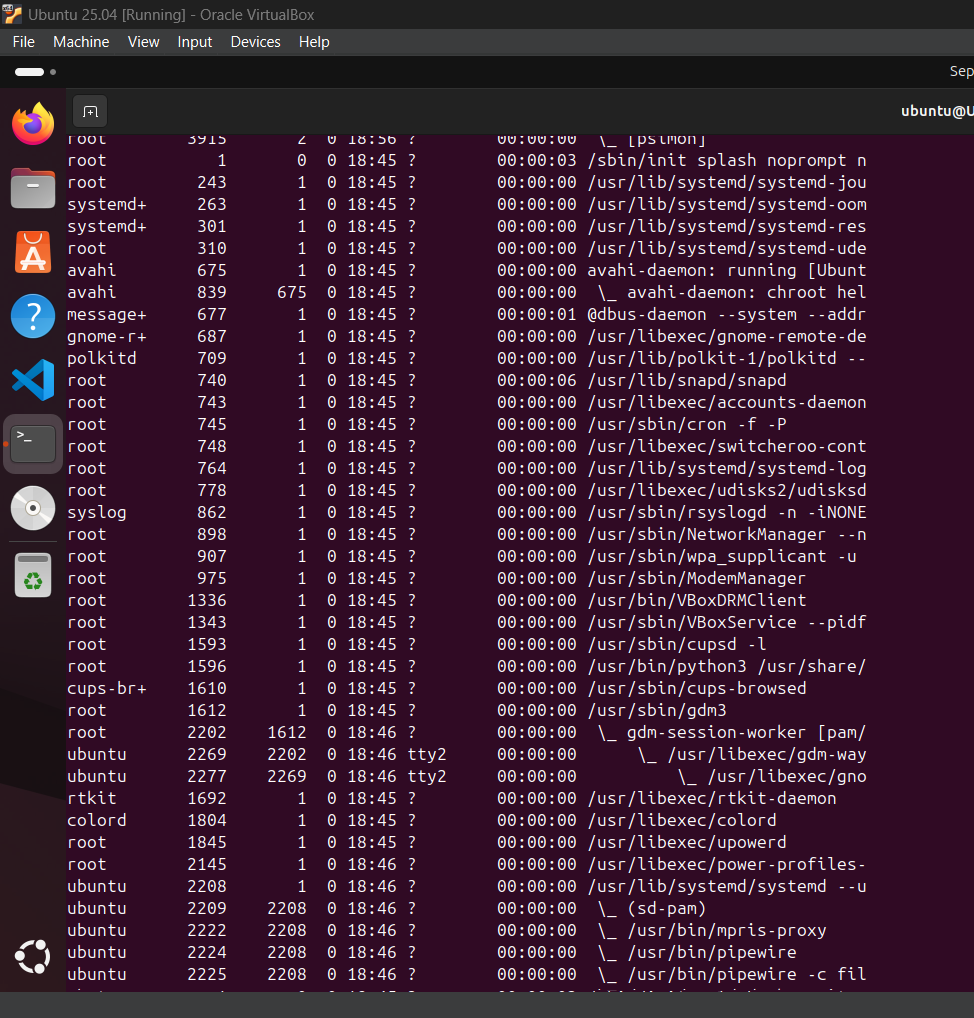
\includegraphics[width=15cm, height=10cm]{png/LinuxProblemSetPicsPNG/TreeView3.png}
        \caption{Part F \#24 Tree View 3}
        \label{fig:partF 24 Tree 3}
    \end{figure}
    \begin{figure}[H]
        \centering
        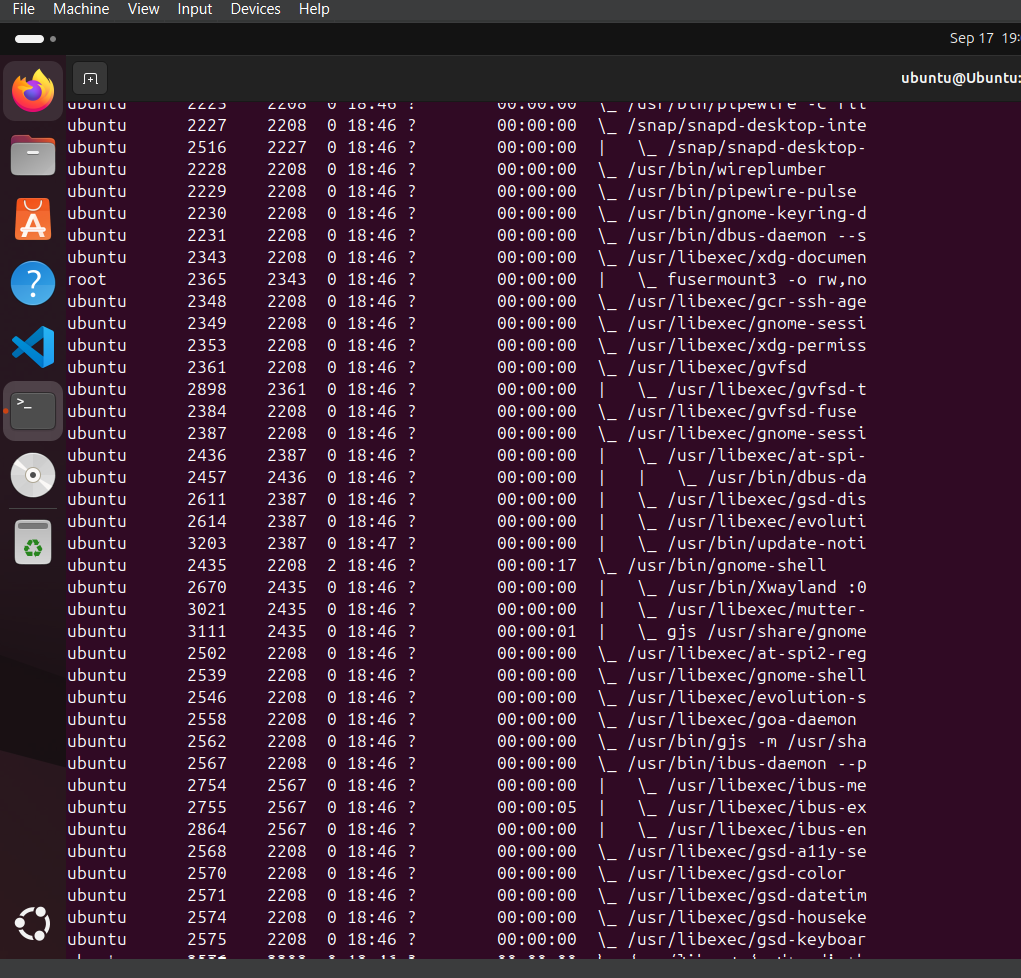
\includegraphics[width=15cm, height=10cm]{png/LinuxProblemSetPicsPNG/TreeView4.png}
        \caption{Part F \#24 Tree View 4}
        \label{fig:partF 24 Tree 4}
    \end{figure}
    \begin{figure}[H]
        \centering
        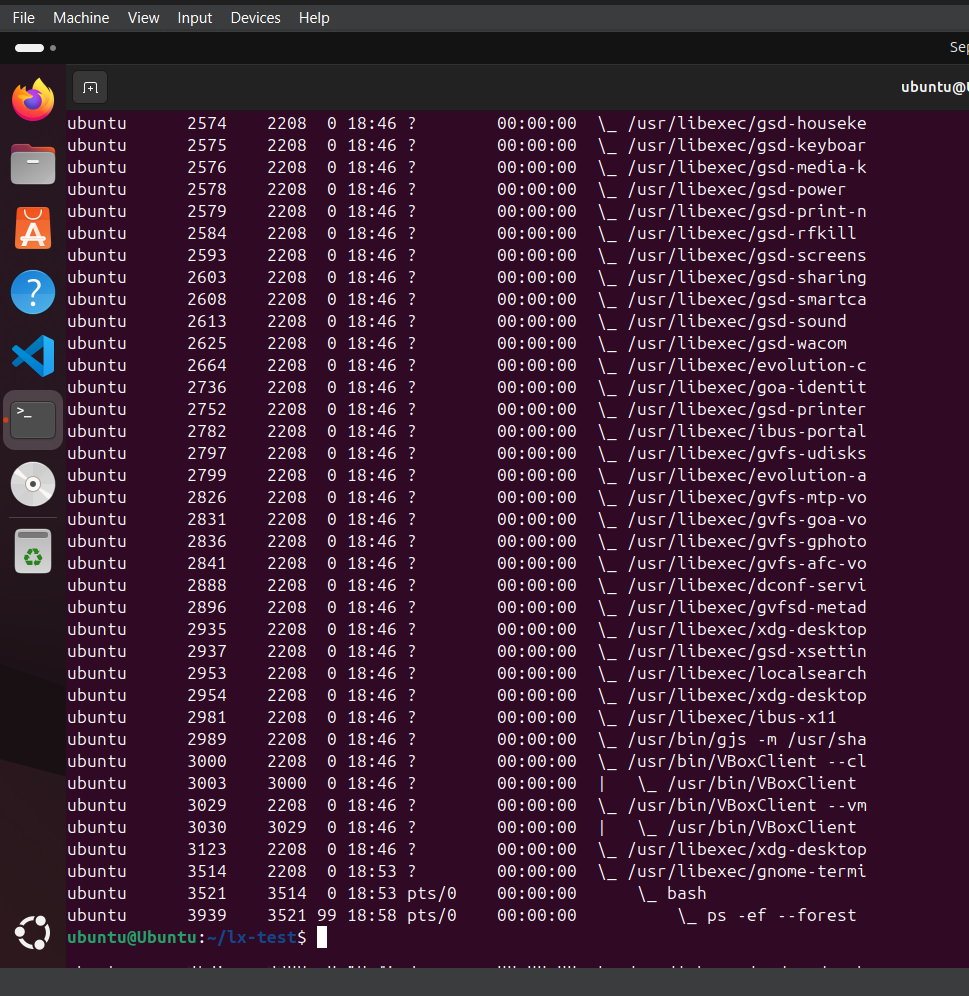
\includegraphics[width=15cm, height=10cm]{png/LinuxProblemSetPicsPNG/TreeView5.png}
        \caption{Part F \#24 Tree View 5}
        \label{fig:partF 24 Tree 5}
    \end{figure}
    
    \item 25: 
     \begin{figure}[H]
        \centering
        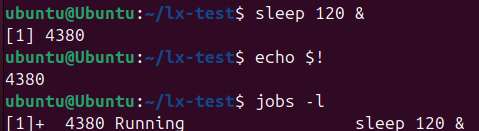
\includegraphics[width=10cm, height=5cm]{png/LinuxProblemSetPicsPNG/PartF25.png}
        \caption{Part F \#25 Sleep 120 in the background and its PID}
        \label{fig:partF 25}
    \end{figure}
    
    \item 26: 
    \begin{figure}[H]
        \centering
        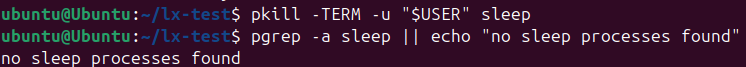
\includegraphics[width=15cm, height=4cm]{png/LinuxProblemSetPicsPNG/PartF26.png}
        \caption{Part F \#26 TERM signal}
        \label{fig:partF 26}
    \end{figure}
    
    \item 27: 
     \begin{figure}[H]
        \centering
        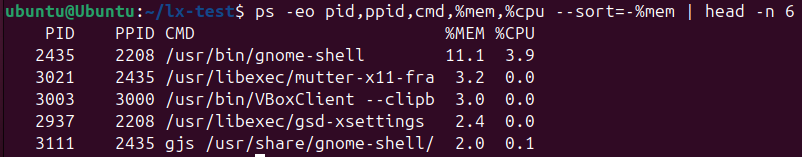
\includegraphics[width=15cm, height=4cm]{png/LinuxProblemSetPicsPNG/PartF27.png}
        \caption{Part F \#27 Top 5 Processes}
        \label{fig:partF 27}
    \end{figure}
\end{itemize}

\section{Part G: Archiving \& Compression}
\begin{itemize}
    \item 28: 
    \begin{lstlisting}[language=Bash]
        tar czf src.tar.gz
    \end{lstlisting}
    \item 29: 
    \begin{lstlisting}[language=Bash]
        tar -tf src.tar.gz
    \end{lstlisting}
    \item 30: 
    \begin{lstlisting}[language=Bash]
        tar -xzf src.tar.gz -C tmp src/file2.txt
    \end{lstlisting}
    \begin{figure}[htp]
    \centering
    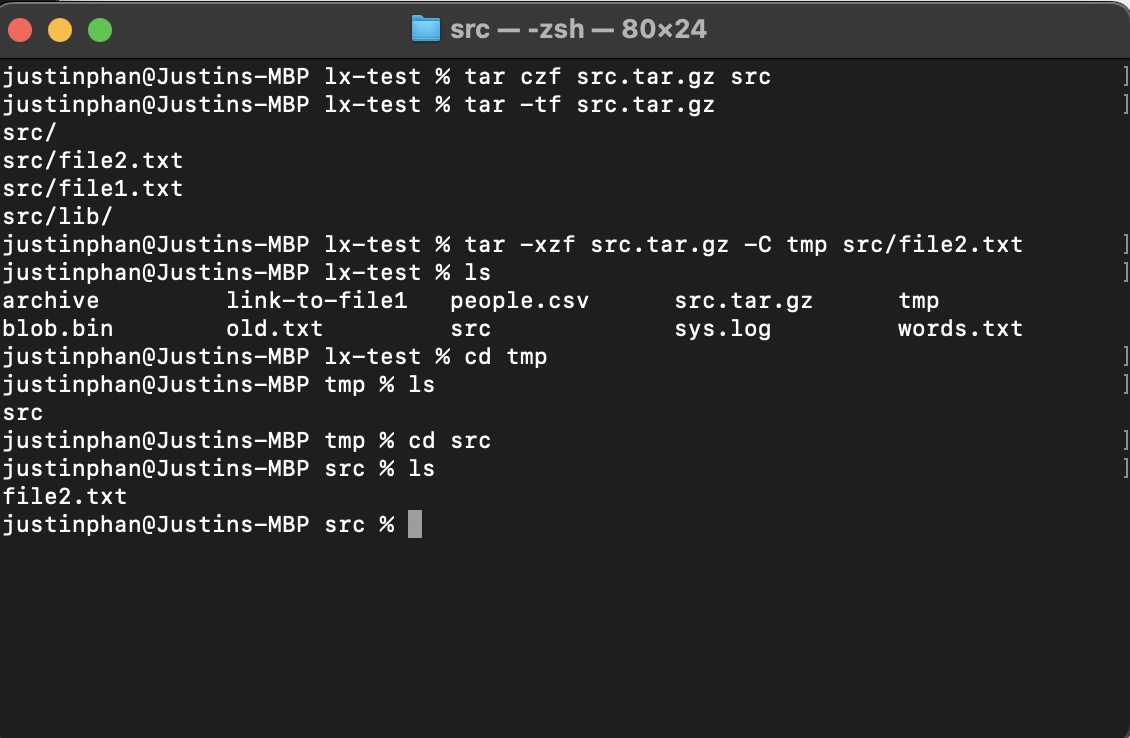
\includegraphics[width=15cm, height=10cm]{png/LinuxProblemSetPicsPNG/part_g.png}
    \caption{Part G Terminal Output}
    \label{fig:part G}
\end{figure}
\end{itemize}

\section{Part H: Networking \& System Info}
\begin{itemize}
    \item 31:
     \begin{figure}[H]
        \centering
        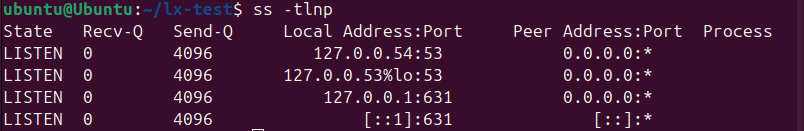
\includegraphics[width=15cm, height=4cm]{png/LinuxProblemSetPicsPNG/PartH31.png}
        \caption{Part H \#31 TCP sockets with associated PIDs }
        \label{fig:partH 31}
    \end{figure}
    
    \item 32: 
     \begin{figure}[H]
        \centering
        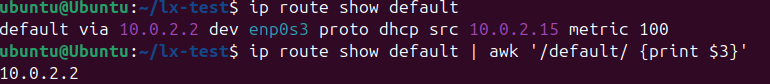
\includegraphics[width=15cm, height=4cm]{png/LinuxProblemSetPicsPNG/PartH32.png}
        \caption{Part H \#32 Default Route (gateway) in a concise form}
        \label{fig:partH 32}
    \end{figure}
    
    \item 33: 
     \begin{figure}[H]
        \centering
        
\includegraphics[width=15cm, height=4cm]{png/LinuxProblemSetPicsPNG/PartH33.png}
        \caption{Part H \#33 Kernel name, Release, and Machine Architecture}
        \label{fig:partH 33}
    \end{figure}
    
    \item 34: 
     \begin{figure}[H]
        \centering
        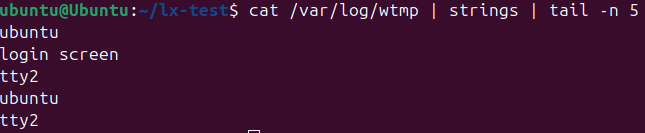
\includegraphics[width=15cm, height=4cm]{png/LinuxProblemSetPicsPNG/PartH34.png}
        \caption{Part H \#34 Last 5 successful logins on the system}
        \label{fig:partH 34}
    \end{figure}

\end{itemize}

\section{Part I: Package \& Services (Debian/Ubuntu)}
\begin{itemize}
    \item 35: 
    \begin{lstlisting}[language=Bash]
         brew list --versions coreutils
    \end{lstlisting}
    \begin{figure}[htp]
    \centering
    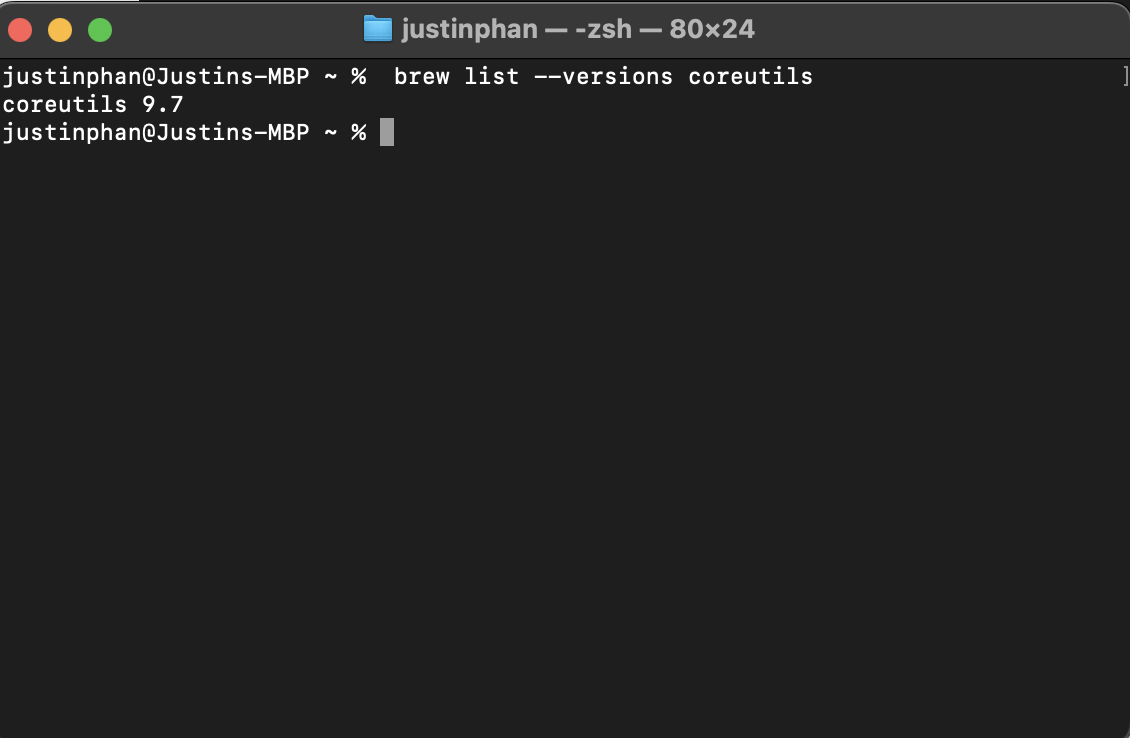
\includegraphics[width=15cm, height=10cm]{png/LinuxProblemSetPicsPNG/part_i_35.png}
    \caption{Part I \#35 Terminal Output showing the installed version of package coreutils}
    \label{fig:part I 35}
\end{figure}
    \item 36: 
    \begin{lstlisting}[language=Bash]
        brew search ripgrep
    \end{lstlisting}
    \begin{figure}[htp]
    \centering
    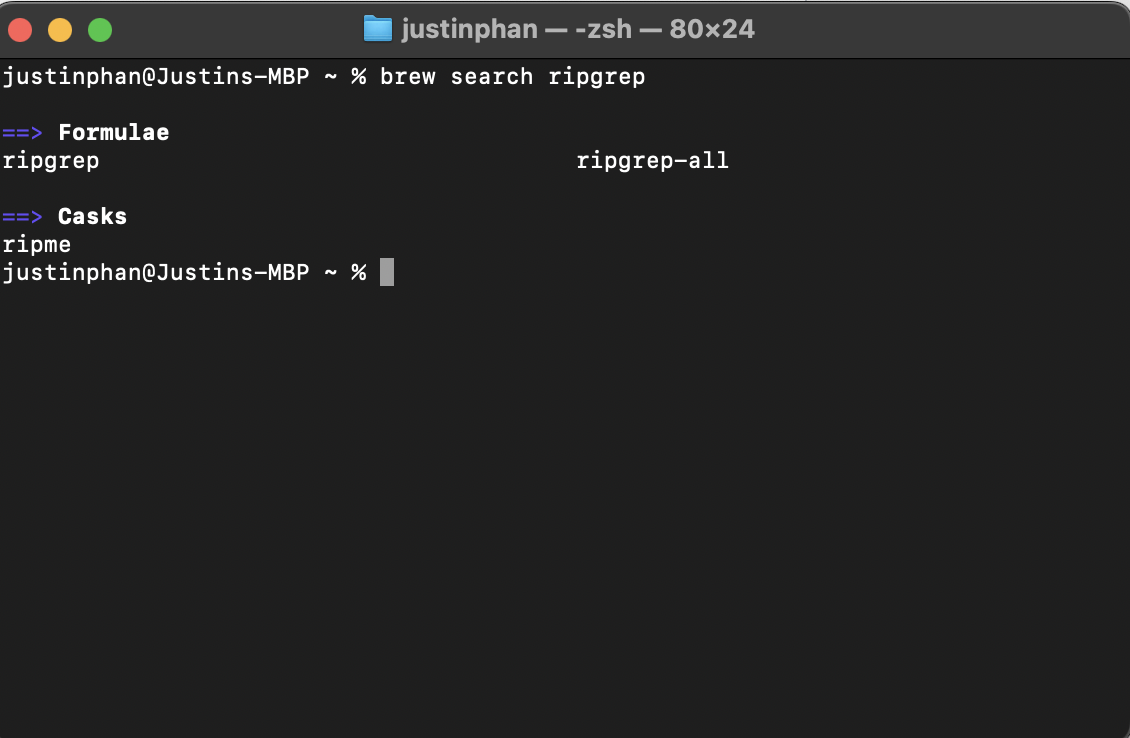
\includegraphics[width=15cm, height=10cm]{png/LinuxProblemSetPicsPNG/part_i_36.png}
    \caption{Part I \#36 Terminal Output showing all available packages whose names contain ripgrep}
    \label{fig:part I 36}
\end{figure}
    \item 37: 
    \begin{lstlisting}[language=Bash]
        systemctl status cron | grep "Active."
    \end{lstlisting}
    \begin{figure}[htp]
    \centering
    
\includegraphics[width=16cm, height=4cm]{png/LinuxProblemSetPicsPNG/part_i_37.png}
    \caption{Part I \#37 Terminal Output}
    \label{fig:part I 37}
\end{figure}
\end{itemize}

\section{Part J: Bash \& Scripting}
\begin{itemize}
    \item 38: 
     \begin{figure}[H]
        \centering
        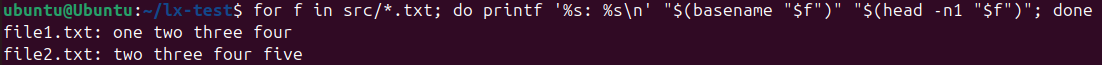
\includegraphics[width=12cm, height=2cm]{png/LinuxProblemSetPicsPNG/PartI38.png}
        \caption{Part J \#38 One-liner that loops over}
        \label{fig:partJ 38}
    \end{figure}
    \item 39: 
     \begin{figure}[H]
        \centering
        
\includegraphics[width=15cm, height=2cm]{png/LinuxProblemSetPicsPNG/PartI39.png}
        \caption{Part J \#39 A command that exports CSV rows}
        \label{fig:partJ 39}
    \end{figure}
    \item 40: 
     \begin{figure}[H]
        \centering
        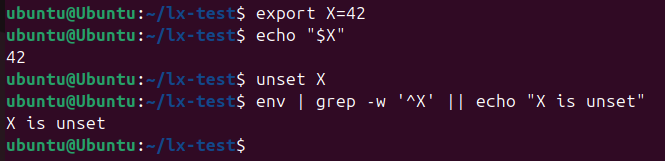
\includegraphics[width=15cm, height=4cm]{png/LinuxProblemSetPicsPNG/PartI40.png}
        \caption{Part J \#40 Create a variable X with value 42}
        \label{fig:partJ 40}
    \end{figure}
\end{itemize}

